\section{Experiments}

In this section, we present the experimental setup, results, and corresponding analysis.

\begin{table*}[h]
    \centering
    %\resizebox{.95\columnwidth}{!}{
    \begin{tabular}{l|cccc}
        \toprule
        Model & RMSE $\downarrow$ &  RMAE $\downarrow$ &  PCC $\uparrow$ &  SRCC $\uparrow$ \\
        \midrule 
        % ICNet & 0.112 & 0.295 & 0.839 & 0.816 \\  % batch size=32
        ICNet & 0.118 & 0.303 & 0.821 & 0.794 \\  % batch size=64
        ViT & 0.097 & 0.273 & 0.883 & 0.874  \\ 
        % Naive-VLISA (ViLT) & 0.111 & 0.288 & 0.842 & 0.842  \\
        Naive VLISA (ViLT) & 0.105 & 0.279 & 0.862 & 0.855 \\ % 1e-4
        Naive VLISA (BERT) & 0.094 & 0.267 & 0.892 & 0.886  \\ 			
        Naive VLISA (Longformer) & \textbf{0.092} & \textbf{0.259} & \textbf{0.895} & \textbf{0.888}  \\			
        % CoT-VLISA (ViLT) & 0.118 & 0.300 & 0.820 & 0.801  \\ 
        CoT VLISA (ViLT) & 0.118 & 0.298 & 0.820 & 0.809 \\ % 1e-4
        CoT VLISA (BERT) & 0.109 & 0.288 & 0.855 & 0.849  \\ 
        CoT VLISA (Longformer) & 0.105 & 0.281 & 0.862 & 0.846  \\ 
        \bottomrule
\end{tabular}
\caption{Performance of different methods on the Entity Complexity Scoring task.
$\uparrow$ indicates that the larger the value, the better.
$\downarrow$ indicates that the smaller the value, the better.
% \KZ{Highlight those best performing numbers in the two tables?}
}
\label{entity_reg}
\end{table*}

\begin{table*}[h]
    \centering
    %\resizebox{.95\columnwidth}{!}{
    \begin{tabular}{l|cccc}
    \toprule
    Model & RMSE  $\downarrow$ &  RMAE  $\downarrow$ &  PCC $\uparrow$ &  SRCC $\uparrow$ \\
    \midrule 
    % ICNet & 0.182 & 0.378 & 0.626 & 0.614 \\   % batch size=32
    ICNet & 0.188 & 0.382 & 0.601 & 0.594 \\  % batch size=64
    ViT & 0.168 & 0.367 & 0.693 & 0.674  \\
    % Naive-VLISA (ViLT) & 0.158 & 0.352 & 0.736 & 0.727  \\
    Naive VLISA (ViLT) & 0.153 & 0.347 & 0.754 & 0.740  \\ % 1e-4
    Naive VLISA (BERT) & 0.146 & 0.338 & 0.780 & 0.761  \\
    Naive VLISA (Longformer) & \textbf{0.141} & 0.328 & 0.798 & 0.786  \\
    % CoT-VLISA (ViLT) & 0.150 & 0.338 & 0.770 & 0.762  \\
    CoT VLISA (ViLT) & 0.147 & 0.336 & 0.776 & 0.762  \\ % 1e-4
    CoT VLISA (BERT) & 0.147 & 0.330 & 0.793 & 0.785  \\
    CoT VLISA (Longformer) & \textbf{0.141} & \textbf{0.319} & \textbf{0.801} & \textbf{0.791}  \\
    \bottomrule
\end{tabular}
\caption{Performance of different methods on the Semantic Complexity Scoring task.}
\label{semantic_reg}
\end{table*}


\begin{table*}[h]
    \centering
    %\resizebox{.95\columnwidth}{!}{
    \begin{tabular}{l|c|cccc}
    \toprule
    Model & CoT Feature & RMSE $\downarrow$ &  RMAE $\downarrow$ &  PCC $\uparrow$ &  SRCC $\uparrow$ \\
    \midrule 
    % Naive VLISA (BERT) & 0.146 & 0.338 & 0.780 & 0.761  \\
                     & CoRs + Description & 0.147 & 0.330 & 0.793 & 0.785  \\
    CoT VLISA (BERT) & w/o CoRs & 0.147 & 0.336 & 0.779 & 0.768 \\
                     & w/o Description & 0.148 & 0.330 & 0.780 & 0.775 \\
    \hline
    % Naive VLISA (Longformer) & 0.141 & 0.328 & 0.798 & 0.786  \\
                           & CoRs + Description & 0.141 & 0.319 & 0.801 & 0.791  \\
    CoT VLISA (Longformer) & w/o CoRs & 0.141 & 0.326 & 0.798 & 0.778 \\
                           & w/o Description & 0.142 & 0.327 & 0.797 & 0.792 \\
    \bottomrule
\end{tabular}
\caption{Ablation study of CoT VLISA on the Semantic Complexity Scoring task.}
\label{ablation}
\end{table*}


%\subsection{Setup}

\paragraph{Models}
For Vision models, we use ICNet~\cite{ic9600} and ViT~\cite{vit} as our baseline models. 
ICNet is a model designed for ICA task. 
ViT is a classic vision model. 
For VLISA, we use GPT-4o~\cite{gpt4} to extract features from the image and use ViLT~\cite{Kim2021ViLTVT}, BERT~\cite{devlin-etal-2019-bert}, and Longformer~\cite{Beltagy2020Longformer} as the Discriminator. 
% and GPT-4o~\cite{gpt4} 

\paragraph{Implementation Details}
We implement the models described in this paper using PyTorch~\cite{torch} and Transformers~\cite{wolf-etal-2020-transformers}.
Each model is trained and evaluated on a single NVIDIA A10 GPU.
We train the ICNet according to the settings in the original paper.
For ViT, ViLT, BERT, and Longformer, we train them for 20 epochs with batch size 16. 
The maximum text input length for ViLT and BERT is set to 512 tokens.
Note that since the max maximum text input length of pre-trained ViLT (\textit{vilt-b32-mlm}) is 40, we randomly initialize its position embeddings.
BERT is fine-tuned based on \textit{bert-base-uncased}.
The maximum input length of Longformer was set to 1024 tokens, and it is fine-tuned on \textit{longformer-base-4096}.
To save GPU memory, Longformer is trained with fp16 16-bit (mixed) precision.
These models are trained and evaluated on our training and test set. 


% The learning rate of ViT is 1e-4.
% The learning rate of BERT is 2e-5.
% The learning rate of Longformer is (2e-5, 5e-5)

\paragraph{Evaluation Metrics}

Following~\citet{ic9600}, we use Root Mean Square Error (RMSE), Root Mean Absolute Error (RMAE), Pearson Correlation Coefficient (PCC), and Spearman's Rank Correlation Coefficient (SRCC) as our evaluation metrics.
The formulas for calculating RMSE and RMAE are

\begin{equation}
RMSE = \sqrt{ \frac{1}{n} \sum\nolimits_{i=1}^{n} (x_i - y_i)^2 }
\end{equation}

and

\begin{equation}
RMAE = \sqrt{ \frac{1}{n} \sum\nolimits_{i=1}^{n} | x_i - y_i |},
\end{equation}
where $n$ is the sample size,  $x_i$ and $y_i$ represent the $i$th label and  predicted score. 

The PCC is defined as

\begin{equation}
r_{xy} = \frac{\displaystyle\sum\nolimits_{i=1}^{n}(x_i-\overline{x})(y_i-\overline{y})}{\sqrt{\displaystyle\sum\nolimits_{i=1}^{n}(x_i-\overline{x})^2}\sqrt{\displaystyle\sum\nolimits_{i=1}^{n}(y_i-\overline{y})^2}},
\end{equation}
where $\overline{x}$ and $\overline{y}$ are the means of $\mathbf{x}$ and $\mathbf{y}$.

The formula of SRCC is 

\begin{equation}
r_s = 1 - \frac{6 \sum_{i=1}^{n} d_i^2}{n(n^2 - 1)},
\end{equation}
where $d_i=R(x_i)-R(y_i)$, $R(x_i)$ and $R(y_i)$ are the ranks of the $i$th image when labels and predicted scores are sorted in descending order.

\paragraph{Results}





Table~\ref{entity_reg} shows the results of Entity Complexity Scoring task.
We can see that the transformer-based vision model ViT is better than the CNN-based ICNet.
Naive VLISA with a pre-trained language model as the Discriminator shows competitive and slightly better performance compared to ViT.
Naive VLISA also shows better performance than CoT VLISA.
The possible reason for the better performance of Naive VLISA is that features extracted by Naive VLISA tend to focus more on describing the content at the entity level within the image.
Conversely, the feature extractor in CoT VLISA extracts higher-level semantic information from the image, but it overlooks some entities.

Table~\ref{semantic_reg} shows the results of Semantic Complexity Scoring task.
We can see that predicting Semantic Score is more challenging than predicting Entity Score and traditional vision models cannot perform well on this task.
Naive VLISA shows obviously better performance than ViT and ICNet.
The possible reason is that with GPT-4o extracting semantic information from the images, the Discriminator in VLISA can perform score prediction at a higher semantic level.
Consistent with the previous hypothesis, CoT VLISA shows better performance than Naive VLISA on this task.
Furthermore, by comparing the performance differences between the VLISA (ViLT) and vision models on the two tasks, we can observe the importance of introducing the language modality for the Semantic Complexity Scoring task.

Generally speaking, Naive VLISA can perform well on both the two sub-tasks of ISA task, CoT VLISA can further improve the performance on the Semantic Complexity Scoring task.

% \KZ{From the results, I think what we want to advocate is Naive VLISA for entity score and CoT VLISA for semantic score. We need to argue why this is the case, not just from the numbers but give some reasons behind.}
% This is consistent with the findings above that features extracted by Naive-VLISA tend to focus more on describing the content at the entity level within the image, while CoT-VLISA extract features on the semantic level.





\paragraph{Ablation Study}

 % the ablation study of CoT VLISA.
CoRs and the description are the two main parts extracted by the Feature Extractor of CoT VLISA, so we validate their effectiveness in this section.
Table~\ref{ablation} shows when either CoRs or the description are removed from the extracted text features, the performance decreases, which demonstrates the necessity of both these two designs in CoT VLISA. 

% \MY{say that 1. Performance gain brought by language reasoning CoT is consistent across different base models (BERT vs. Longformer), 2. you have to be careful as results on different metrics say different things, why don't we remove the part of comparison on w/o cor/description? or just illustrate one feature.}



\section{Analysis}

\begin{figure*}[ht]
    \centering
    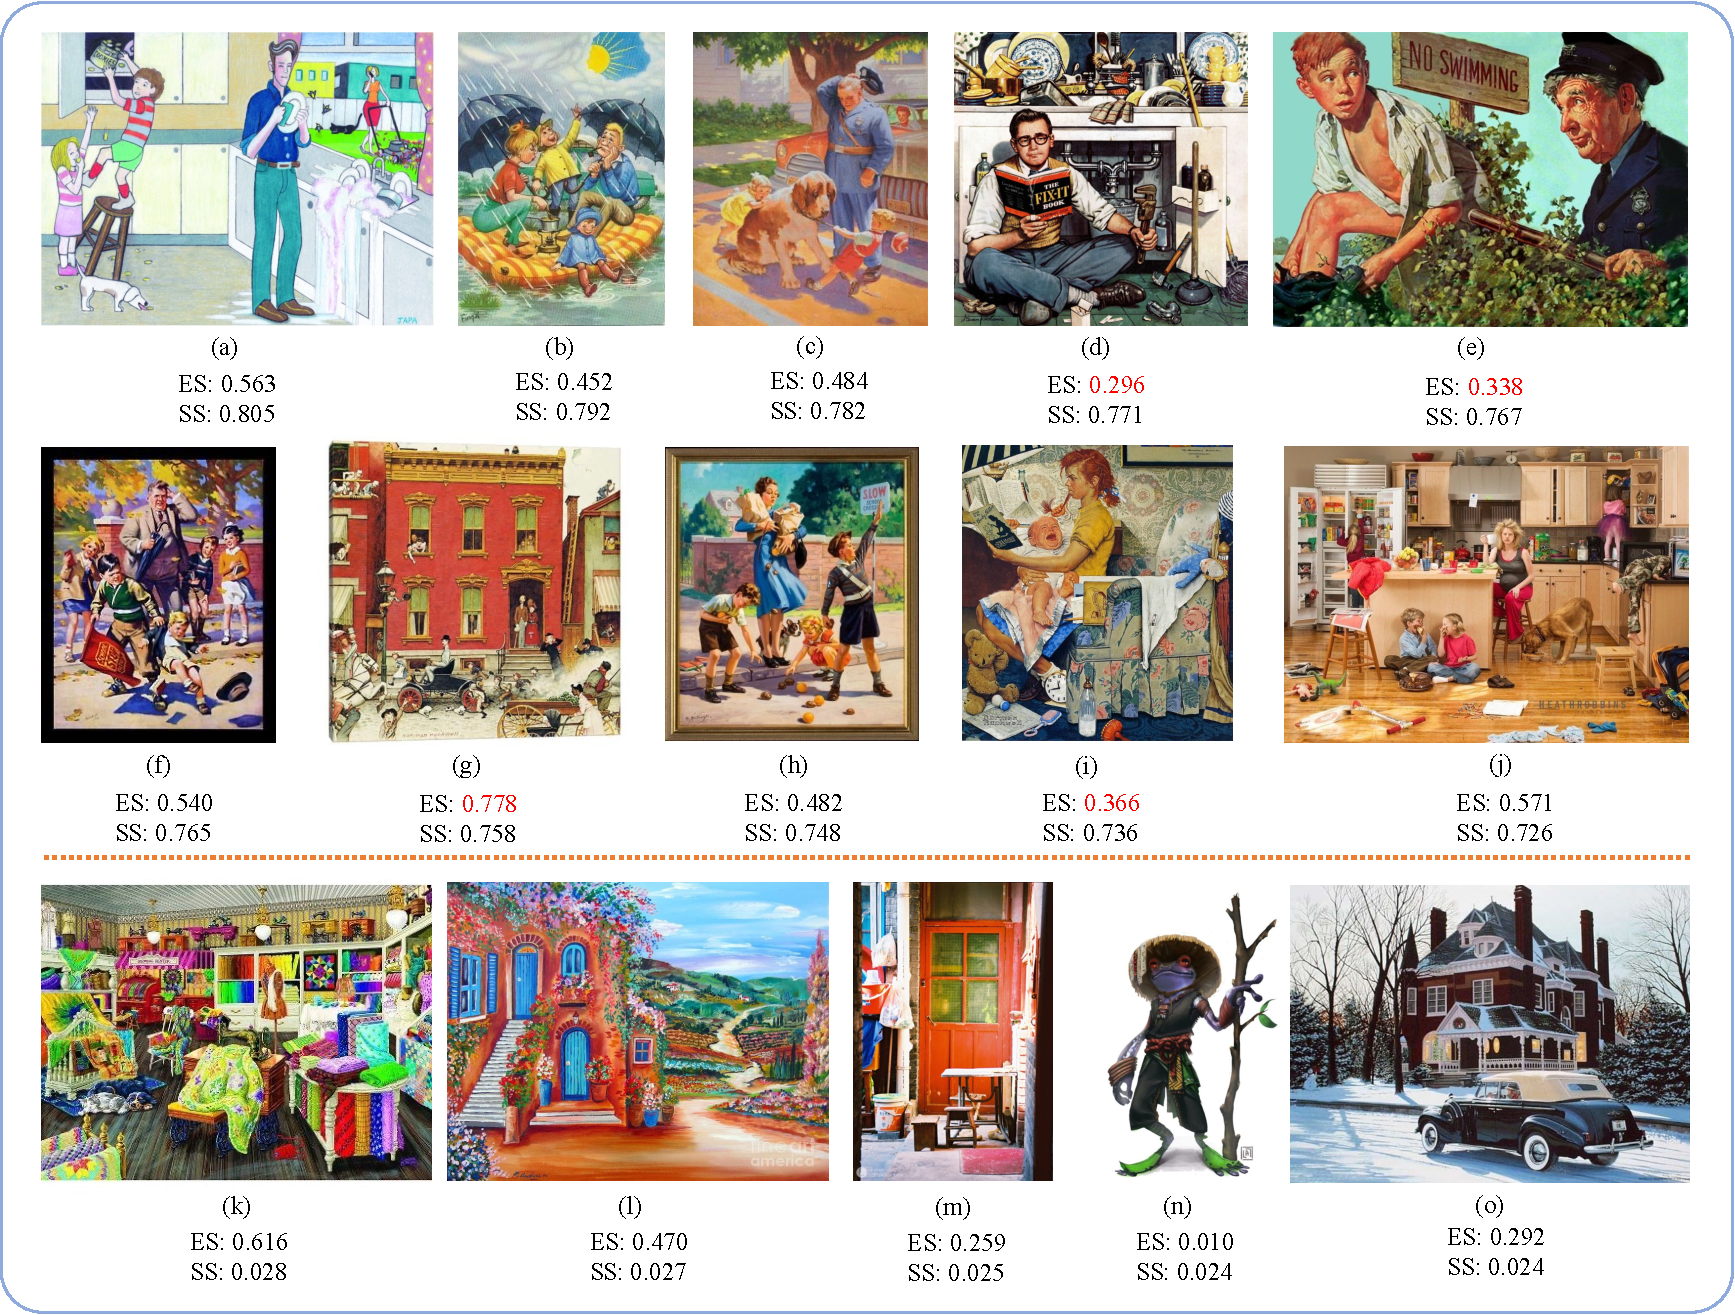
\includegraphics[scale=0.5]{figs/pred_case3.pdf}
    \caption{Case study. ES and SS stand for Entity Score and Semantic Score predicted by Naive VLISA (Longformer) respectively. The samples above the orange line are those with the highest Semantic Scores, sorted in descending order. The samples below the orange line are those with the lowest Semantic Scores. Red Entity Scores indicate that they are either too high or too low.
    % \KZ{What about those scores in red?}
    }
    \label{pred_case}
\end{figure*}

When applying VLISA to find semantically rich images, we recommend first locating images with high Semantic Scores. 
Then, users can further select images that match their application scenario according to the Entity Score.
Figure~\ref{pred_case} shows some samples with their scores predicted by Naive VLISA (Longformer).
According to the design guidelines of the Cookie Theft picture, we prefer images with higher Semantic Scores and Entity Scores between 0.4 and 0.6.
Based on Figure~\ref{pred_case}, we can see that images with the highest Semantic Scores generally tell an interesting story, i.e. they contain more semantic information.

Interestingly, without including the Cookie Theft image in the training set, the image with the highest Semantic Score is Cookie Theft (Figure~\ref{pred_case} (a)).
Based on Entity Score, we can further filter out images with too few or too many entities. 
For instance, Figure~\ref{pred_case} (d), (e), and (i) contain fewer entities and Figure~\ref{pred_case} (g) contains more entities than we expect.
That is, the remaining images above the orange line are more preferred by the Cookie Theft design principles.
Note that although many images in our dataset are not real-world images, our VLISA method can still give appropriate Semantic Scores to these real-world images.
For example, the image (j) in Figure~\ref{pred_case} has a high Semantic Score and it is actually quite similar to the Cookie Theft semantically.
This demonstrates that by extracting semantic information in language form, our Feature Extractor can help the Discriminator avoid the influence of types or styles of images in some content.

For images with the lowest Semantic Scores under the orange line, there is either a single action (Figure~\ref{pred_case} (n-o)) or no event at all (Figure~\ref{pred_case} (k-m)) in the image, which is consistent with our annotation design.
These samples show VLISA can successfully help us collect images with rich semantics. 
